\documentclass[12pt, letterpaper]{article}
\date{\today}
\usepackage[margin=1in]{geometry}
\usepackage{amsmath}
\usepackage{hyperref}
\usepackage{cancel}
\usepackage{amssymb}
\usepackage{fancyhdr}
\usepackage{pgfplots}
\usepackage{booktabs}
\usepackage{pifont}
\usepackage{amsthm,latexsym,amsfonts,graphicx,epsfig,comment}
\pgfplotsset{compat=1.16}
\usepackage{xcolor}
\usepackage{tikz}
\usetikzlibrary{shapes.geometric}
\usetikzlibrary{arrows.meta,arrows}
\newcommand{\Z}{\mathbb{Z}}
\newcommand{\N}{\mathbb{N}}
\newcommand{\R}{\mathbb{R}}
\newcommand{\Po}{\mathcal{P}}

\author{Alex Valentino}
\title{Homework 6}
\pagestyle{fancy}
\renewcommand{\headrulewidth}{0pt}
\renewcommand{\footrulewidth}{0pt}
\fancyhf{}
\rhead{
	Homework \\
	292
}
\lhead{
	Alex Valentino\\
}
\begin{document}
\begin{enumerate}
	\item[6]
	\begin{enumerate}
		\item[a]
			Let $y(t) = x'(t), \Vec{x} = (x(t),y(t))$.  Therefore $\Vec{x}' = (x',y') = (y,-\frac{k}{m}x - \frac{a}{m}y) = \begin{bmatrix} 0 & 1 \\ -\frac{k}{m} & -\frac{a}{m}\end{bmatrix} \Vec{x}$.  Thus $B = \begin{bmatrix} 0 & 1 \\ -\frac{k}{m} & -\frac{a}{m}\end{bmatrix}$.
		\item[b]
			\begin{itemize}
				\item Suppose $(\frac{a}{m})^2 = \frac{4k}{m}$ (critically dampened). We must compute $e^{tB}$. Thus $0 = det(B - \lambda \mathbb{I}_2) = \lambda^2 + \frac{a}{m}\lambda +\frac{k}{m}$, therefore $\lambda = \frac{\frac{-a}{m} \pm \sqrt{(\frac{a}{m})^2 - \frac{4k}{m}}}{2} = \frac{\frac{-a}{m} \pm 0}{2} = \frac{-a}{2m}$.  Thus $\lambda^2 + \frac{a}{m}\lambda +\frac{k}{m} = (\lambda + \frac{a}{2m})^2$.  Therefore $\lambda = \frac{-a}{2m}$ is an eigenvalue with multiplicity 2.  Since we are in $\R^2$, and that is the same as the multiplicity of the eigenvalue then we know that $(B + \frac{a}{2m})^2 \Vec{x} = 0$ for all $\Vec{x} \in \R^2$.  Therefore $e^{tB} = e^{\frac{-a}{2m}t} \sum_{k=0}^1 t^k (B + \frac{a}{2m} \mathbb{I}_2) = e^{\frac{-a}{2m}t} (\mathbb{I}_2 + t \begin{bmatrix} \frac{a}{2m} & 1\\ \frac{-k}{m} &\frac{-a}{2m} \end{bmatrix} ) = e^{\frac{-a}{2m}t} \begin{bmatrix}1 + t\frac{a}{2m} & t\\ \frac{-k}{m}t & 1 - \frac{a}{2m}t \end{bmatrix}$.  
				\item Suppose $(\frac{a}{m})^2 < \frac{4k}{m}$ (under dampened).  We must compute $e^{tB}$.  Since $(\frac{a}{m})^2 < \frac{4k}{m}$ then $(\frac{a}{m})^2 - \frac{4k}{m} = \frac{-\rho^2}{m^2}$.  Therefore $\lambda =  \frac{\frac{-a}{m} \pm \sqrt{(\frac{a}{m})^2 - \frac{4k}{m}}}{2} = \frac{\frac{-a}{m} \pm i\frac{\rho}{m}}{2} = \frac{1}{2m}(-a\pm i \rho)$.  
				Let $\mu_1 = \frac{1}{2m}(-a + i \rho), \mu_2 =\frac{1}{2m}(-a - i \rho) $.  Computing eigenvalues for $\mu_1$ yields $\Vec{v}_1 = (1,\frac{1}{2m} (-a+i \rho))$.    Therefore $z_1 = e^{\mu_1 t} (1,\frac{1}{2m} (-a+i \rho)) = e^{\frac{-a}{2m}t} (\cos(\frac{\rho}{2m}t) + i \sin(\frac{\rho}{2m}t)) (1,\frac{1}{2m} (-a+i \rho)).$  Let $l = \frac{\rho}{2m}$.  \\
				Thus 
				\begin{align*}
				z_1 &= e^{\frac{-a}{2m}t} (\cos(\frac{\rho}{2m}t) + i \sin(\frac{\rho}{2m}t)) (1,\frac{1}{2m} (-a+i \rho)) \\
				&= e^{\frac{-a}{2m}t} (\cos(lt) + i \sin(lt)) (1,\frac{1}{2m} (-a+i \rho)) \\
				&=  e^{\frac{-a}{2m}t} (\cos(lt),\frac{1}{2m} (-a\cos(lt)  - \rho \sin(lt))) + i e^{\frac{-a}{2m}t} (\sin(lt),\frac{1}{2m} (-a\sin(lt)  + \rho \cos(lt)))
\end{align*}								
			Since we have a single complex solution, then we have the two real solutions forming the columns of $M(t)$:
				$$
				e^{\frac{-a}{2m}t}\begin{bmatrix}
				\cos(lt) & \sin(lt)\\
				\frac{1}{2m} (-a\cos(lt) - \rho \sin(lt) & \frac{1}{2m} (\rho \cos(lt)-	a\sin(lt)				
				\end{bmatrix}
				$$
				Since $M(0) = \begin{bmatrix} 1 & 0 \\ \frac{-a}{2m} & \frac{\rho}{2m} \end{bmatrix}$ then $M^{-1} (0) = \begin{bmatrix}
			1 & 0 \\ \frac{a}{\rho} & \frac{2m}{\rho}	
\end{bmatrix}.				 $ 
			Therefore \begin{align*}
			e^{tB} = M(t) M^{-1}(0) &= e^{\frac{-a}{2m}t}\begin{bmatrix}
				\cos(lt) & \sin(lt)\\
				\frac{1}{2m} (-a\cos(lt) - \rho \sin(lt) & \frac{1}{2m} (\rho \cos(lt)-	a\sin(lt)				
				\end{bmatrix}\begin{bmatrix}
			1 & 0 \\ \frac{a}{\rho} & \frac{2m}{\rho}	
\end{bmatrix}\\ &= e^{\frac{-a}{2m}t} \begin{bmatrix}
	\frac{a}{\rho} \sin(lt) + \cos(lt) & \frac{2m}{\rho} \sin(lt)\\ -\frac{2k}{\rho} \sin(lt) & -\frac{a}{\rho} \sin(lt) + \cos(lt)
\end{bmatrix}. 
			\end{align*}
			\item Suppose $(\frac{a}{m})^2 > \frac{4k}{m}$ (over dampened).  We must compute $e^{tB}$.  Since  $(\frac{a}{m})^2 > \frac{4k}{m}$ then $\lambda = \frac{1}{2m} (-a \pm \rho)$.  Let $\mu_1 =  \frac{1}{2m} (-a + \rho), \mu_2 =  \frac{1}{2m} (-a - \rho)$.  These correspond to the eigenvectors $v_1 = (1,\frac{1}{2m}(-a + \rho)), v_2 = (1,\frac{1}{2m} (-a - \rho))$.  Therefore $z_1 = e^{\frac{1}{2m} (-a + \rho)t} (1, \frac{1}{2m} (-a + \rho)), z_2 = e^{\frac{1}{2m} (-a - \rho)t} (1, \frac{1}{2m} (-a - \rho))$. 
			Therefore 
			$$
			M(t) = e^{\frac{-a}{2m}t} \begin{bmatrix}
			e^{lt} & e^{-lt}\\
			\frac{e^lt}{2m}(\rho - a) & -\frac{e^{-lt}}{2m} (\rho + a)
\end{bmatrix}						
			$$.
			$M^{-1}(0) = \begin{bmatrix}1 & 1\\ \frac{\rho -a}{2m} & \frac{-\rho -a}{2m}	\end{bmatrix}^{-1} = \frac{1}{\rho} \begin{bmatrix} \frac{\rho + a}{2} & -m\\  \frac{\rho - a}{2} & -m \end{bmatrix} $.
			Thus 
			\begin{align*}
			e^{tB} &= M(t)M^{-1}(0)\\
			&= \frac{e^{\frac{-a}{2m}t}}{\rho} \begin{bmatrix}
			e^{lt} & e^{-lt}\\
			\frac{e^lt}{2m}(\rho - a) & -\frac{e^{-lt}}{2m} (\rho + a)
\end{bmatrix} \begin{bmatrix} \frac{\rho + a}{2} & -m\\  \frac{\rho - a}{2} & -m \end{bmatrix}\\
&= \frac{e^{\frac{-a}{2m}t}}{\rho} \begin{bmatrix}
\frac{\rho + a}{2} e^{lt} + \frac{\rho - a}{2}e^{-lt} & -m(e^{lt} + e^{-lt})\\ \frac{1}{2m}(\rho^2 + a^2)(e^{lt} - e^{-lt}) & \frac{\rho + a}{2} e^{lt} - \frac{\rho - a}{2}e^{-lt}
\end{bmatrix}\\
	&= e^{\frac{-a}{2m}t} \begin{bmatrix}
	\frac{a}{\rho} \sinh(lt) + \cosh(lt) & \frac{1}{l} \sinh(lt)\\ \frac{-2k}{\rho} \sinh(lt) & \frac{-a}{\rho} \sinh(lt) + \cosh(lt)
	\end{bmatrix}
			\end{align*}
			\end{itemize}
		
		\item[b(2?)]
			Since $\Vec{x} = e^{tB}\Vec{x}_0$, where $\Vec{x}_0 = (x_0,v_0)$, then $x(t) = e^{\frac{-a}{2m}t}(x_0(1+t\frac{a}{2m}) + v_0 t)$.  We want to find $t$ such that $0 = x(t)$.  Thus we have that $0 = e^{\frac{-a}{2m}t}(x_0(1+t\frac{a}{2m}) + v_0 t)$.  Since $e^{\frac{-a}{2m}t}$ is strictly positive then $0 = x_0(1+t\frac{a}{2m}) + v_0 t$.  This may be rewritten as $ \frac{-x_0}{v_0 + \frac{a}{2m}} = t$.  If this value either diverges or is negative then the solution will not pass through the origin, and if it does we have found an explicit single value for $t$.  Thus there is either one or zero times which $x(t) = 0$.  
		\item[c] Since $\Vec{x} = e^{tB}\Vec{x}_0$, where $\Vec{x}_0 = (x_0,v_0)$, then $x(t) = e^{\frac{-a}{2m}t}(x_0 ( \frac{a}{\rho} \sinh(lt) + \cosh(lt)) + \frac{v_0}{l} \sinh(lt))$.  We want to find when $x(t) = 0$  Since $e^{\frac{-a}{2m}t}$ is strictly positive then we have that $ 0=x_0 ( \frac{a}{\rho} \sinh(lt) + \cosh(lt)) + \frac{v_0}{l} \sinh(lt)$.  Rearrange and assuming that $\frac{x_0 a}{\rho} + \frac{v_0}{l} \neq 0$ we get that $ -(\frac{\frac{x_0 a}{\rho} + \frac{v_0}{l}}{x_0})^{-1} = \tanh(lt)$.  Since $tanh$ is 1-1 then we have a unique $t$ if the value is in the range of $\tanh$, if not then the function doesn't pass through the origin.  If $\frac{x_0 a}{\rho} + \frac{v_0}{l} = 0$ then we have $0= x_0 \cosh(x)$, similarly, since $\text{arcosh}$ is 1-1 then we have a unique $t$ at which the function passes through the origin.  Therefore $x(t) = 0$ occurs at most once for all parameters.  
		\item[d] Since $\Vec{x} = e^{tB}\Vec{x}_0$, where $\Vec{x}_0 = (x_0,v_0)$, then $x(t) = e^{\frac{-a}{2m}t}(x_0 ( \frac{a}{\rho} \sin(lt) + \cos(lt)) + \frac{v_0}{l} \sin(lt))$. We want to find when $x(t) = 0$.  Since $e^{\frac{-a}{2m}t}$ is strictly positive then we have that $ 0=x_0 ( \frac{a}{\rho} \sin(lt) + \cos(lt)) + \frac{v_0}{l} \sin(lt)$.  Rearrange and assuming that $\frac{x_0 a}{\rho} + \frac{v_0}{l} \neq 0$ we get that $ -(\frac{\frac{x_0 a}{\rho} + \frac{v_0}{l}}{x_0})^{-1} = \tan(lt)$.  Note that since $\tan$ is periodic and $\arctan$ is $1-1$ means that $t = \frac{\pi n + \arctan(-(\frac{\frac{x_0 a}{\rho} + \frac{v_0}{l}}{x_0})^{-1})}{l}$ where $n \in \Z$ are all valid solutions.  If $\frac{x_0 a}{\rho} + \frac{v_0}{l} = 0$ then we have $0= x_0 \cos(x)$, similarly, since $\cos$ is periodic and not the zero function due to $x(t) \neq 0$ then we have $t=\frac{\pi n}{l}$ where $n \in \Z$.  Since all cases have an infinite number of solutions, then $x(t)$ transits the origin an infinite number of times.\newline
		\item[e] 
		\begin{itemize}
			\item Over dampening\\
			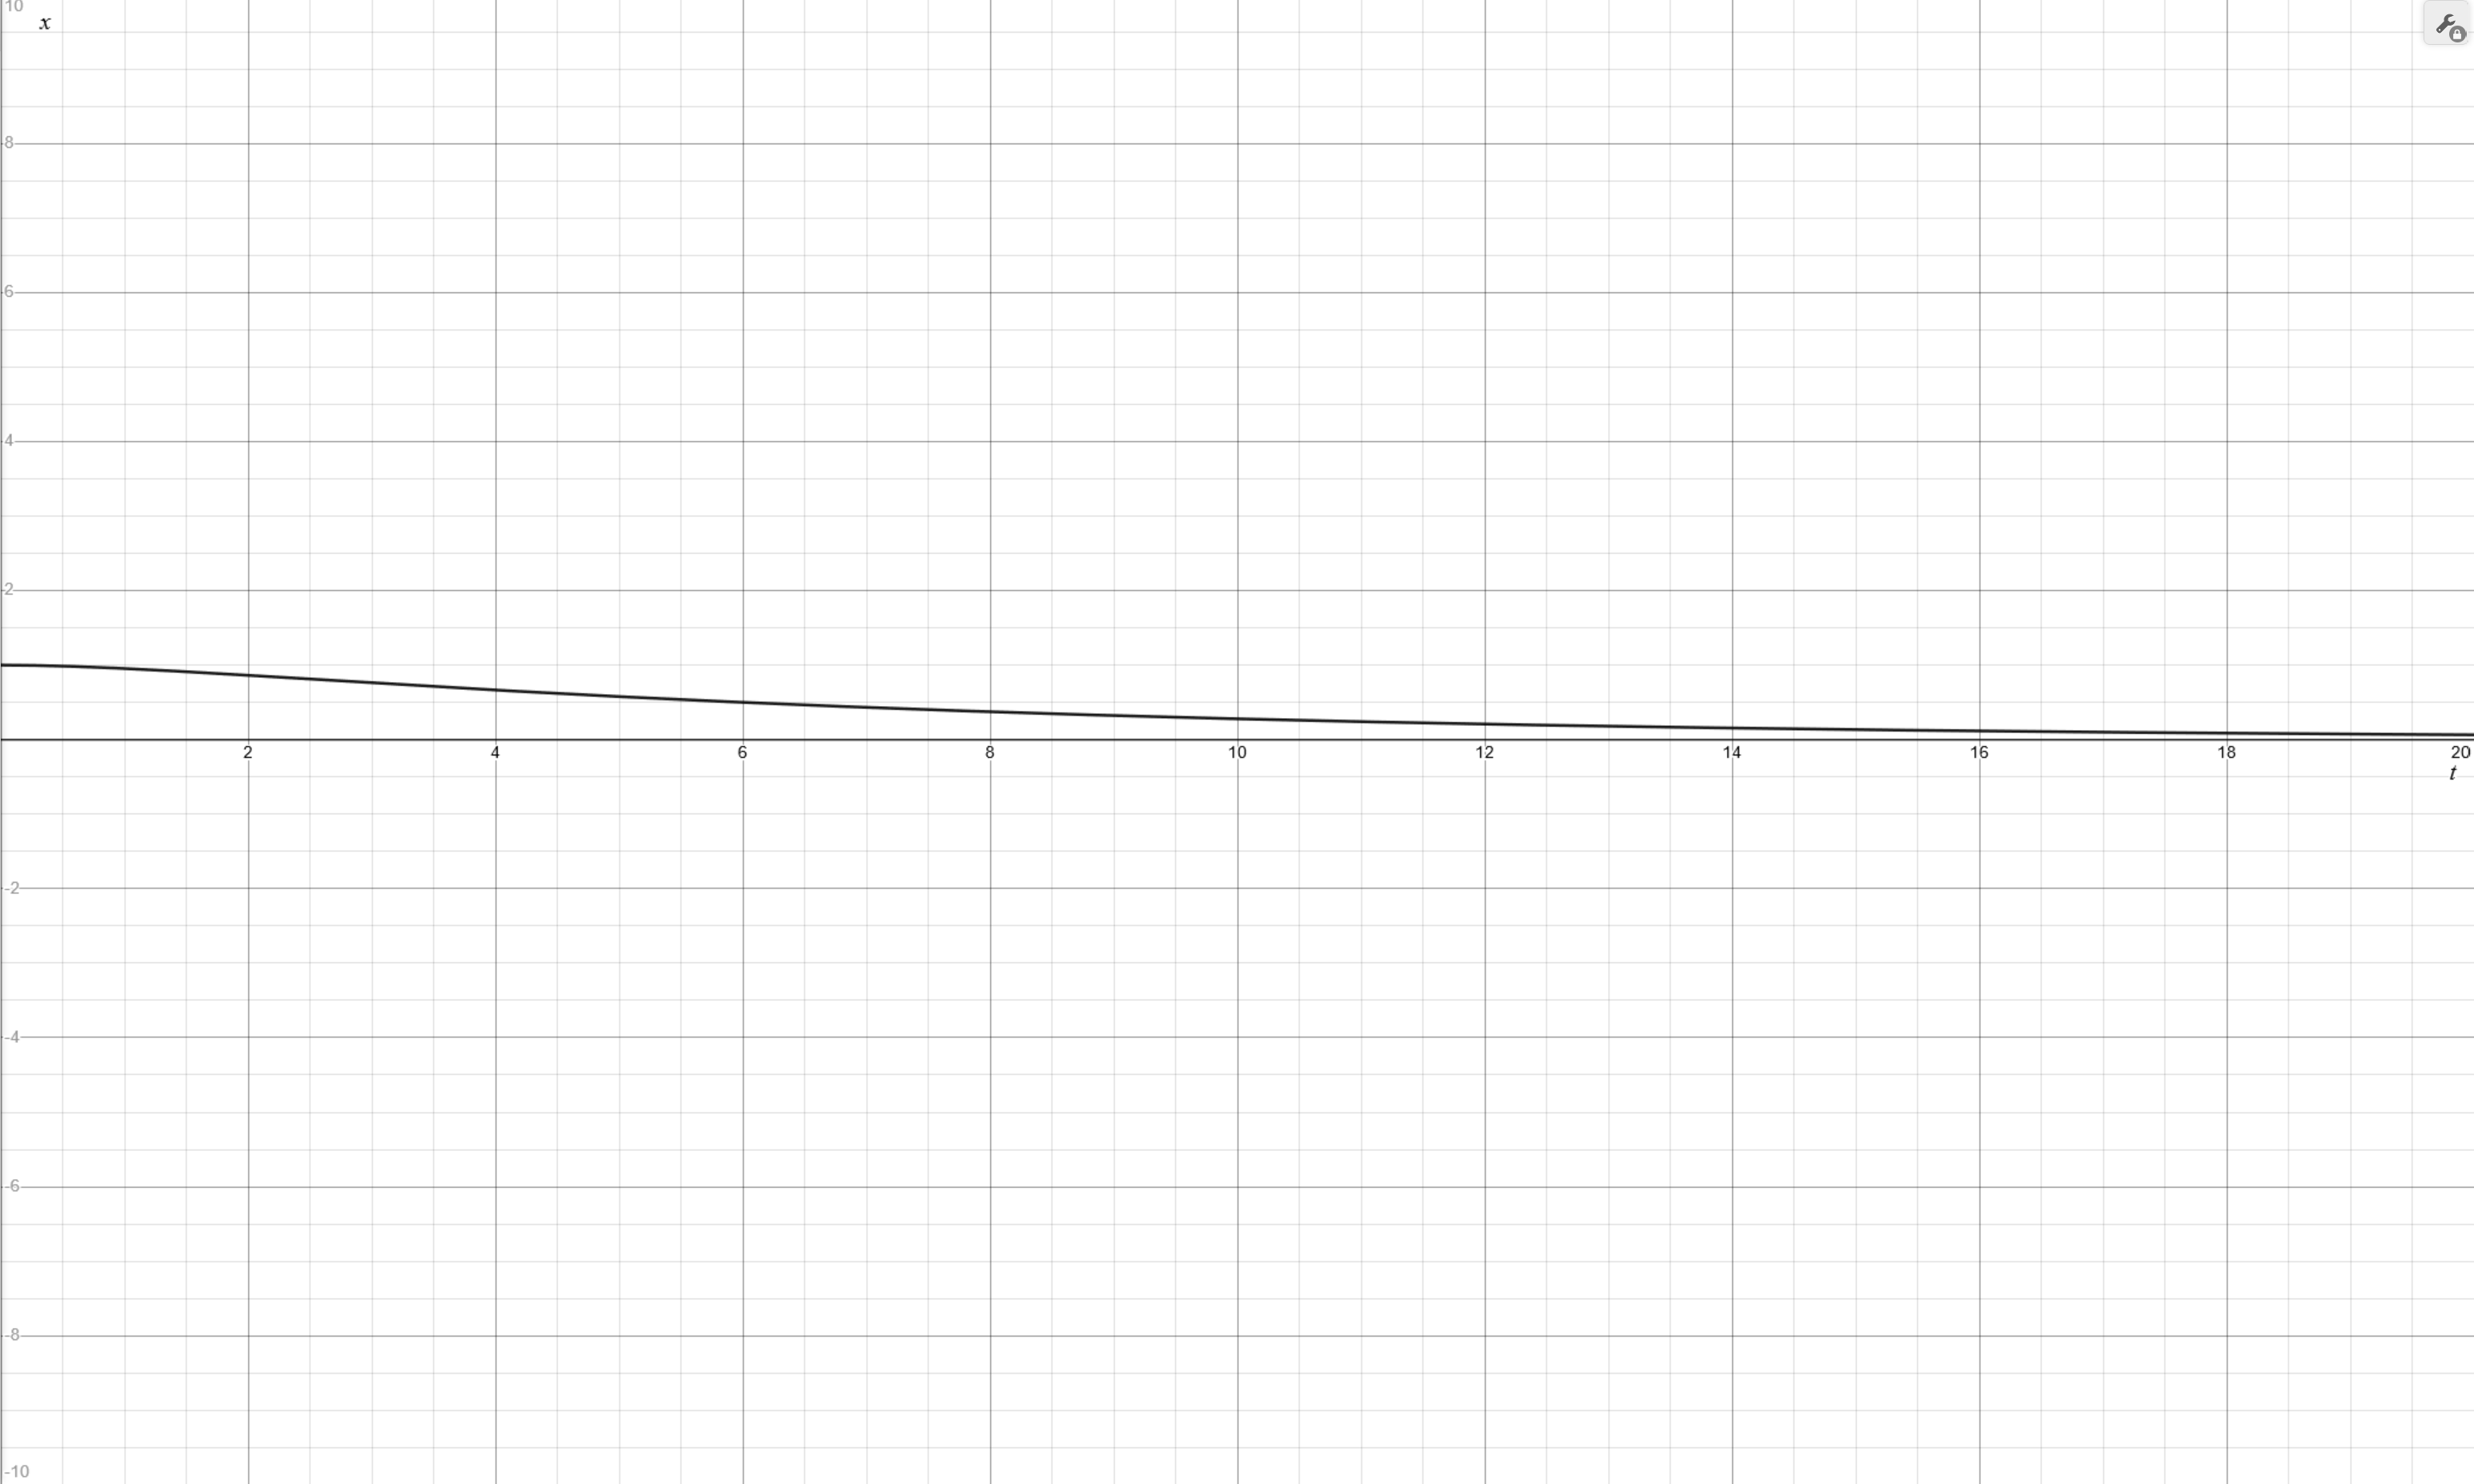
\includegraphics[scale=0.3]{overdamped292hw6}
			\item Under dampening\\
			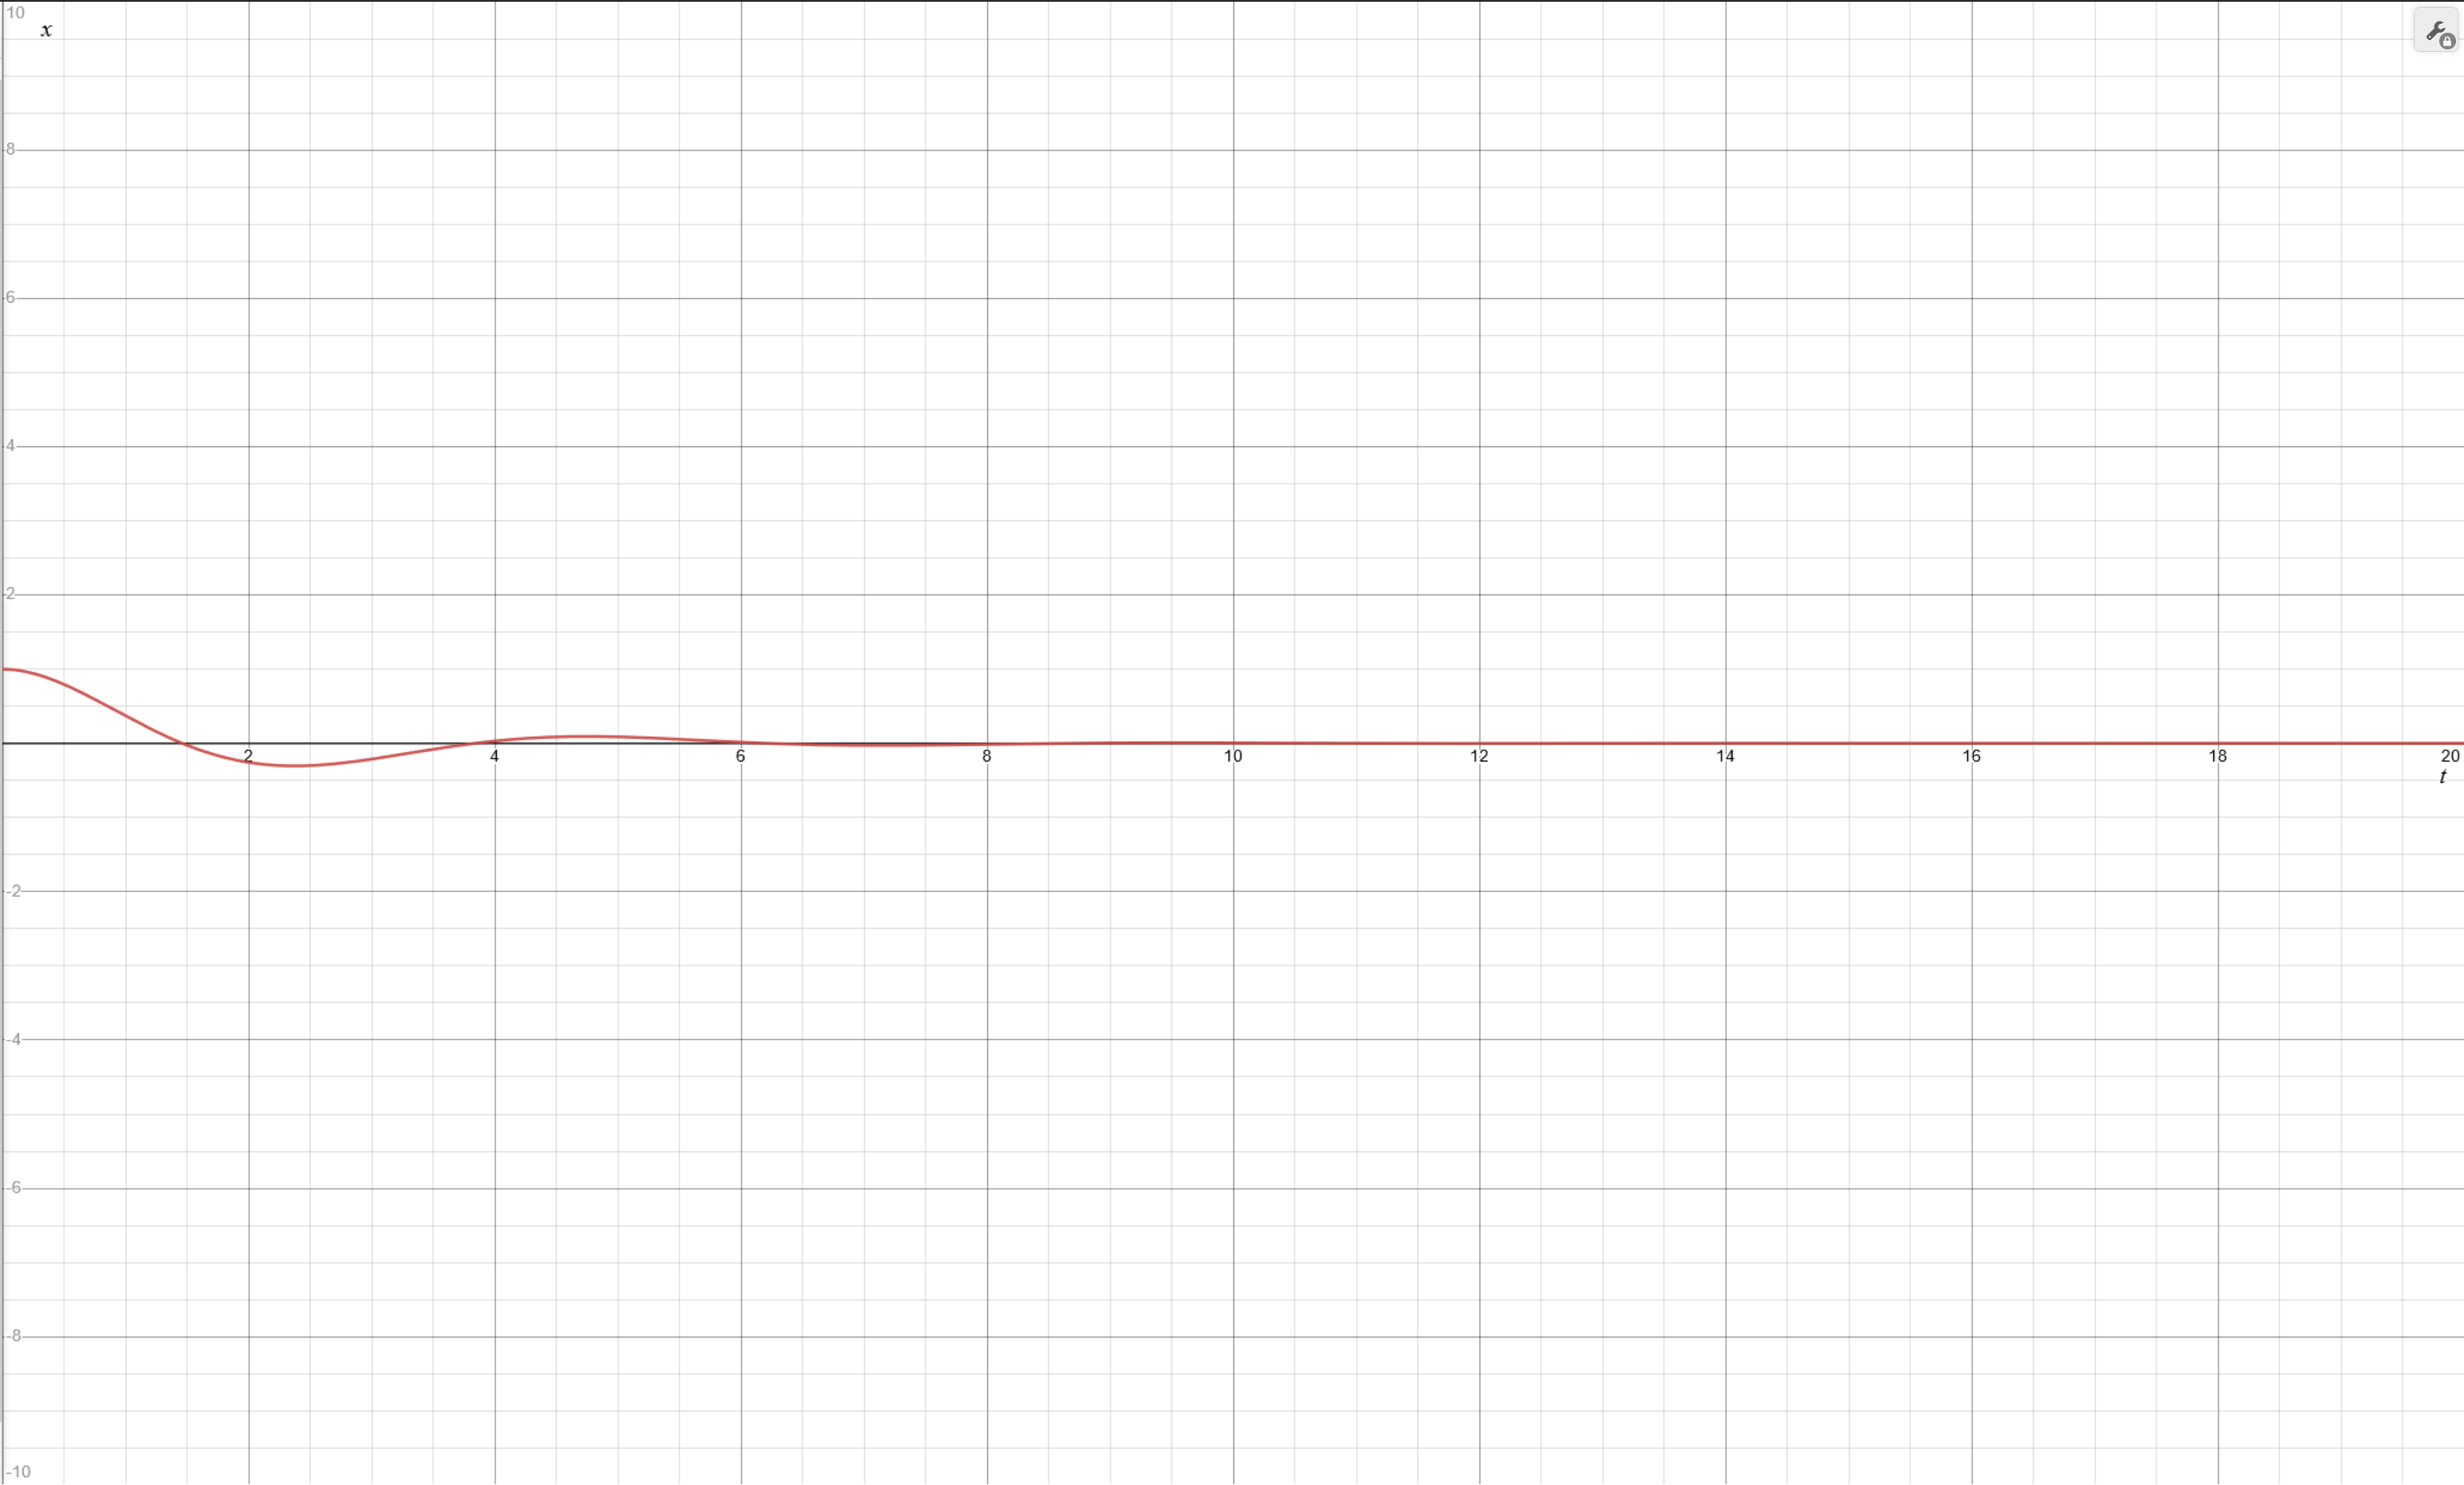
\includegraphics[scale=0.3]{underdamped292hw6}		
			\item Critical dampenening\\
			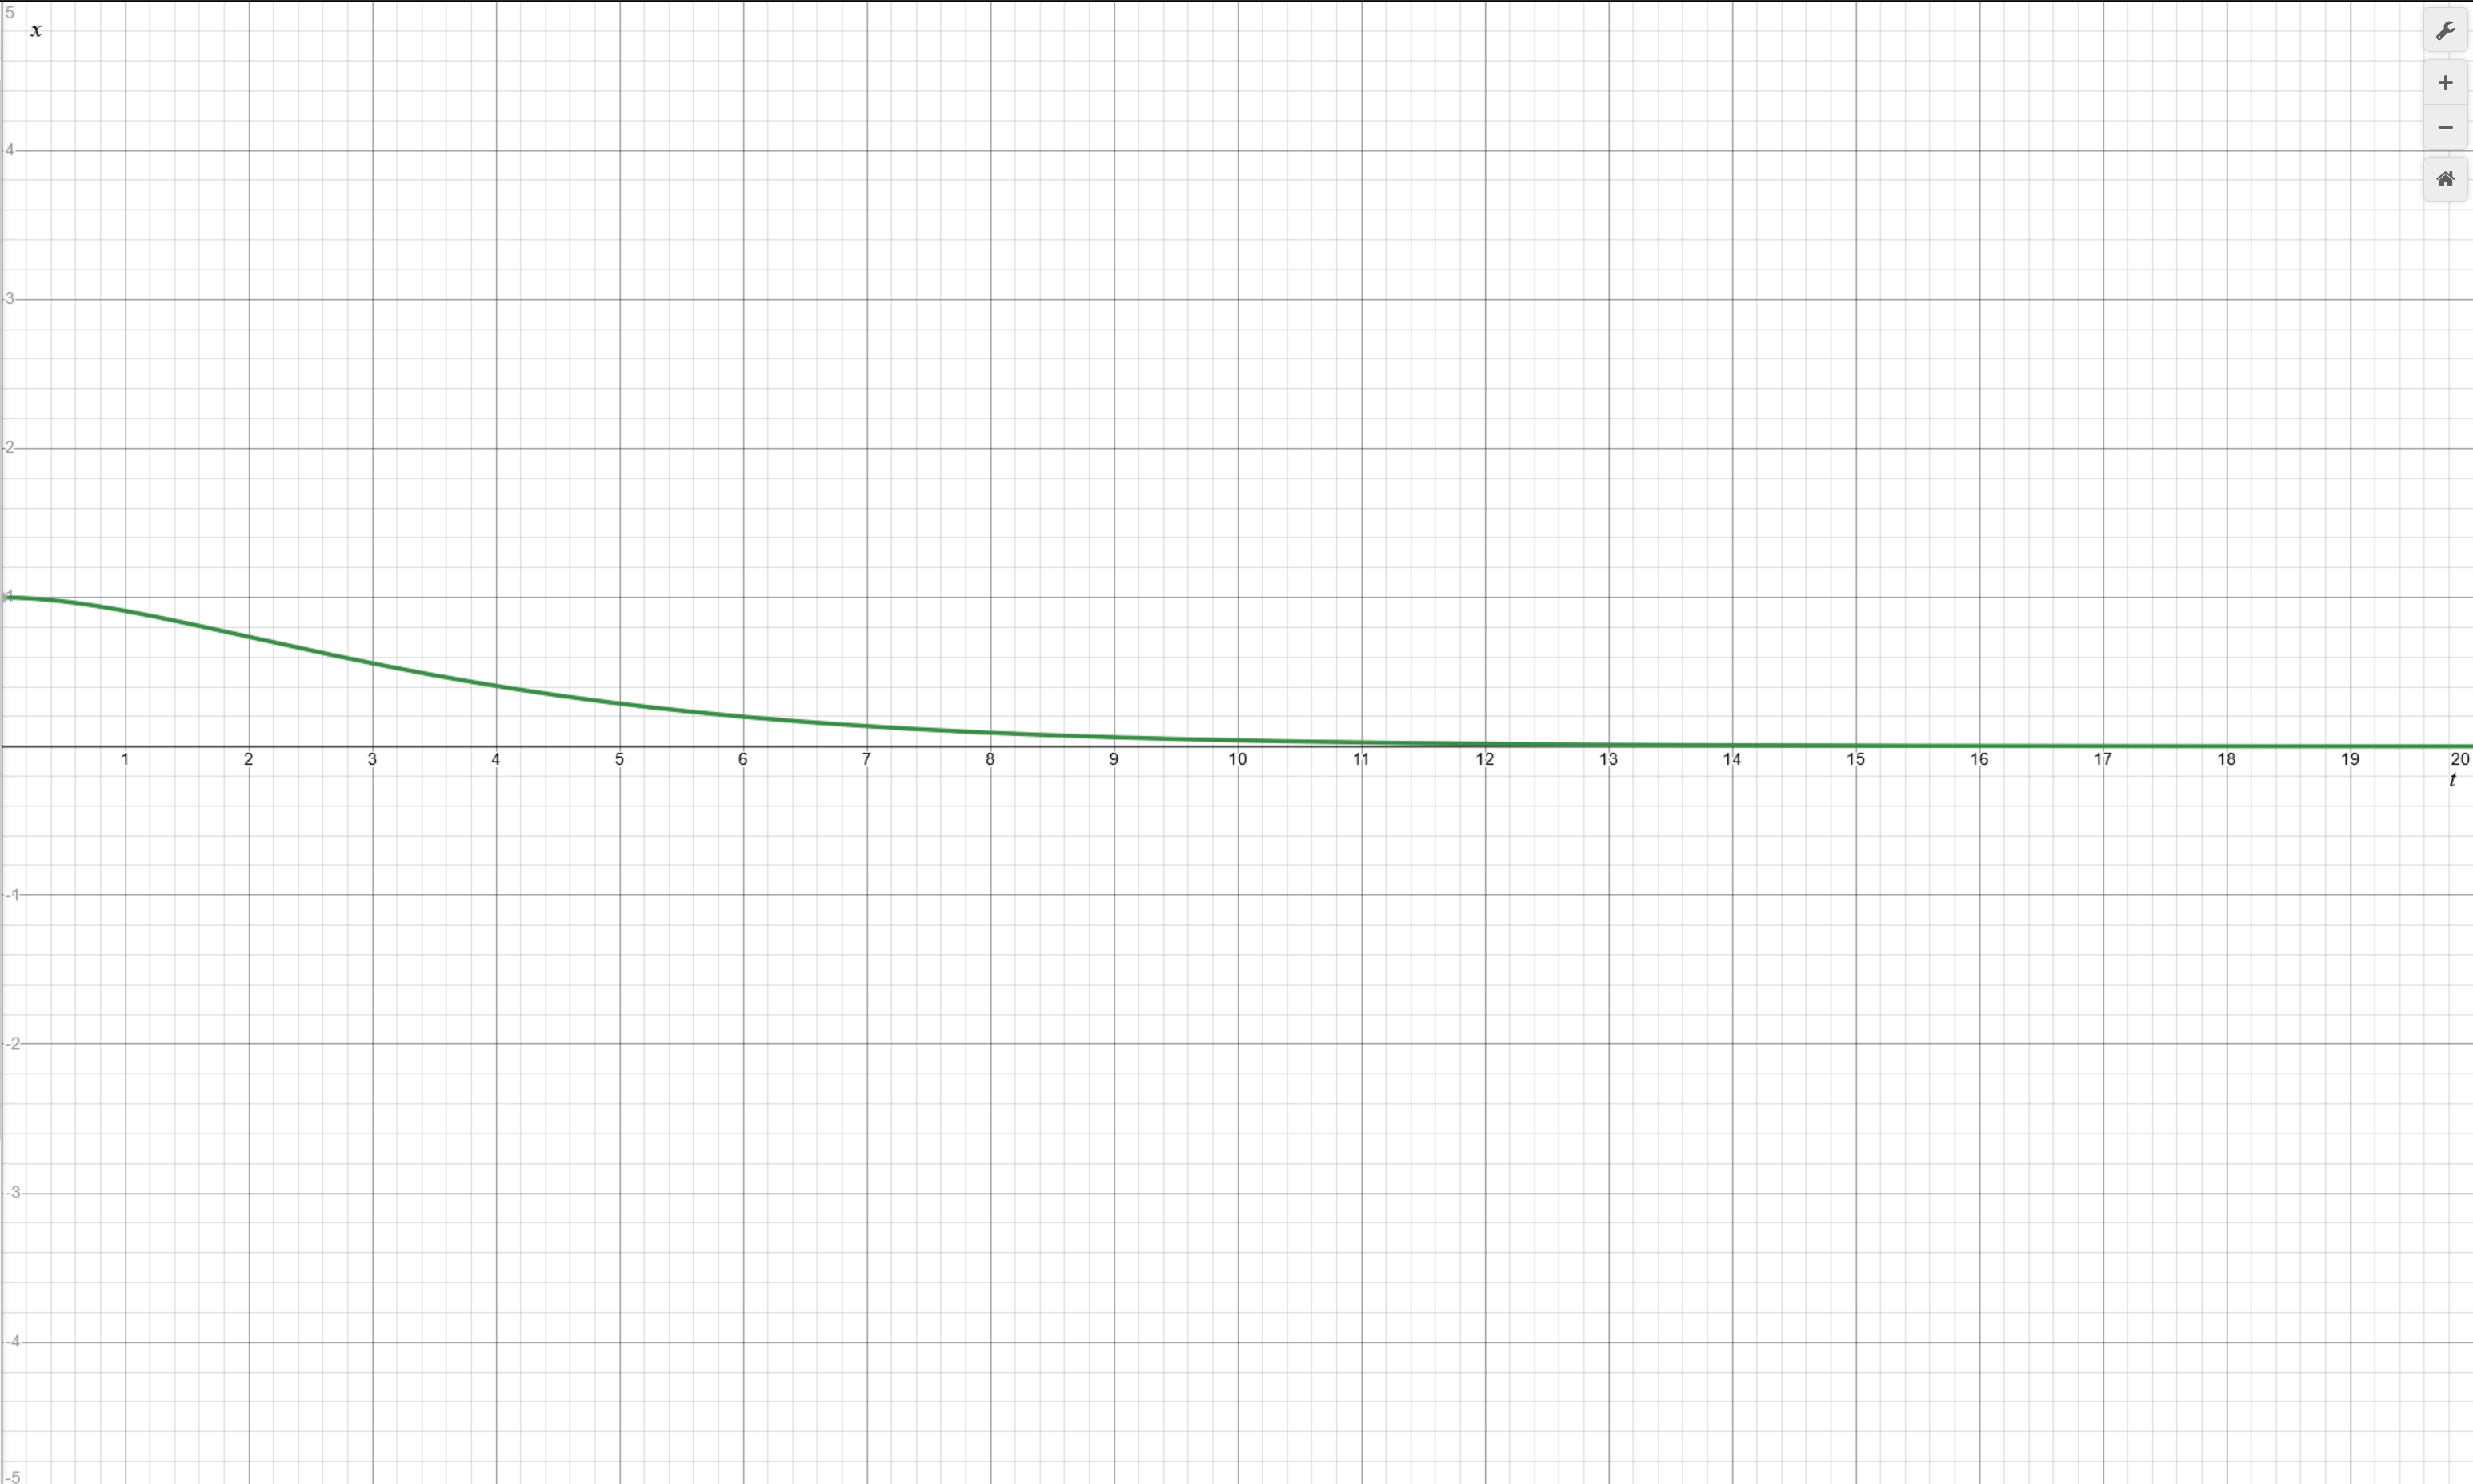
\includegraphics[scale=0.3]{criticallydampened292hw6.png}
		\end{itemize}
	\end{enumerate}
	\item[7] By our previous expression for $\Vec{x}'$, we can define our new $\Vec{x}'(t) = B \Vec{x} (t) + \begin{bmatrix}0 \\ g(t) \end{bmatrix}$. 
		Therefore by Duhamel's formula $\Vec{x} = e^{tB}\Vec{x}_0 + \int_{t_0}^t e^{(t-s)B} \begin{bmatrix}0 \\ g(s) \end{bmatrix}ds$	
	\begin{enumerate}
		\item[a] 
		\begin{itemize}
			\item Suppose $(\frac{a}{m})^2 = \frac{4k}{m}$.  Then our formula becomes 
			\begin{align*}
				 x(t) &= e^{\frac{-a}{2m}t} (x_0(1 + t\frac{a}{2m}) + y_0 t) + \int_{t_0}^t  e^{\frac{-a}{2m}(t-s)}(t-s)\cos(\omega s) ds 
			\end{align*}			  
			\item Suppose $(\frac{a}{m})^2 < \frac{4k}{m}$.  Then our formula becomes 
			$$
							
			$$
		\end{itemize}
	\end{enumerate}
\end{enumerate}
\end{document}